% --- Instruction following and arenas ---
\begin{frame}{MT-Bench: A Small, Open-Ended, Multi-Turn Benchmark}
  \begin{columns}[T,onlytextwidth]
    \column{0.52\textwidth}
      \begin{itemize}\footnotesize\itemsep0.3em
        \item[\textcolor{red}{$\blacktriangleright$}] \textbf{80 questions} in \textbf{8 categories} (10 each): writing, roleplay, extraction, reasoning, math, coding, knowledge~I (STEM), knowledge~II (humanities and social science).
        \item[\textcolor{red}{$\blacktriangleright$}] Every question has \textbf{two turns}: an initial instruction and a follow-up, so the benchmark tests whether the model can stay coherent across a conversation rather than answering one shot.
        \item[\textcolor{red}{$\blacktriangleright$}] Scoring is \textbf{single-answer grading on a 1--10 scale} by GPT-4, averaged over the 160 turns. There is no reference answer for most categories --- which is exactly why a judge is needed.
        \item[\textcolor{red}{$\blacktriangleright$}] 80 questions is tiny. That is a deliberate trade: enough to be judged carefully (and cross-checked against 3{,}000 expert votes) but far too few to resolve small differences. Treat MT-Bench as a \textbf{smoke test}, not a ranking.
        \item[\textcolor{red}{$\blacktriangleright$}] The category breakdown is more informative than the mean: models that look similar overall diverge sharply on math, coding, and reasoning.
      \end{itemize}
    \column{0.46\textwidth}
      \centering
      \vspace{1.0em}
      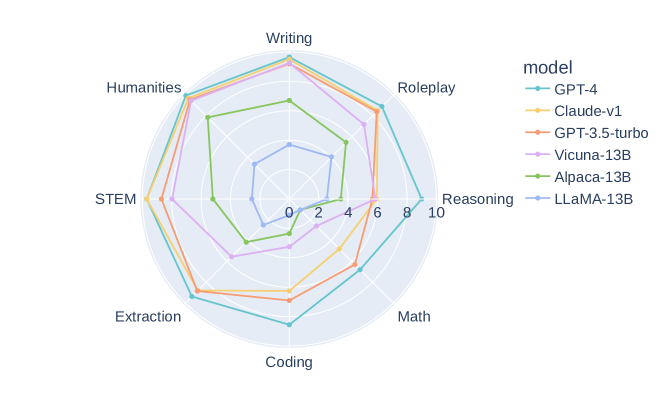
\includegraphics[width=\linewidth,height=0.66\textheight,keepaspectratio]{images/llm-evaluation/mtbench_fig20_category_radar.png}\\[0.2em]
      {\scriptsize ``Category-wise scores of 6 models on MT-bench.'' Zheng et al., ``Judging LLM-as-a-Judge with MT-Bench and Chatbot Arena,'' NeurIPS 2023 Datasets and Benchmarks, \href{https://arxiv.org/abs/2306.05685v4}{arXiv:2306.05685v4}, Figure 20.}
  \end{columns}
\end{frame}

\begin{frame}{Chatbot Arena: Crowdsourced Pairwise Preference}
  \begin{itemize}\itemsep0.05em
    \item[\textcolor{red}{$\blacktriangleright$}] A user types a prompt, sees \textbf{two anonymous models} answer side by side, votes for the better one, and only then learns which was which. Anonymity is what makes the vote a preference rather than a brand survey.
    \item[\textcolor{red}{$\blacktriangleright$}] Scale as reported in the platform paper (January 2024): over \textbf{240{,}000 votes} from about \textbf{90{,}000 users}, covering \textbf{50+ models} and \textbf{100+ languages}. The MT-Bench paper had reported roughly 30{,}000 votes after the first month.
    \item[\textcolor{red}{$\blacktriangleright$}] \textbf{What it buys you:} a live, uncurated prompt distribution that is very hard to contaminate, and preferences from people with an actual task in mind.
    \item[\textcolor{red}{$\blacktriangleright$}] \textbf{What it costs you:} no reproducibility, no ground truth, a self-selected user population, an unknown and drifting prompt mix, and heavy sensitivity to presentation style.
    \item[\textcolor{red}{$\blacktriangleright$}] Because votes are \textbf{pairwise and sparse} --- most model pairs never meet often enough --- the raw win matrix is not a ranking. You need a model to turn comparisons into scores.
  \end{itemize}
  {\scriptsize Chiang et al., ``Chatbot Arena: An Open Platform for Evaluating LLMs by Human Preference,'' ICML 2024, \href{https://arxiv.org/abs/2403.04132v1}{arXiv:2403.04132v1}.}
\end{frame}

\begin{frame}{From Votes to Ratings: Elo, Bradley--Terry, and Error Bars}
  \begin{itemize}\footnotesize\itemsep0.3em
    \item[\textcolor{red}{$\blacktriangleright$}] \textbf{Elo} is an \textit{online} update rule from chess: after each game a player's rating moves by a step proportional to the surprise, with expected score
      \[
        \mathbb{E}[S_A] = \frac{1}{1 + 10^{(R_B - R_A)/400}}.
      \]
      Because it is sequential, the final ratings depend on \textbf{the order the votes arrived in} --- an unattractive property for a leaderboard.
    \item[\textcolor{red}{$\blacktriangleright$}] The arena therefore moved to the \textbf{Bradley--Terry} model, which states the same relationship but fits it \textit{in batch} by maximum likelihood --- it is exactly a logistic regression on model-indicator features:
      \[
        \Pr(i \text{ beats } j) = \sigma(\beta_i - \beta_j) = \frac{e^{\beta_i}}{e^{\beta_i} + e^{\beta_j}}.
      \]
      Ratings no longer depend on vote order, and standard statistical machinery becomes available.
    \item[\textcolor{red}{$\blacktriangleright$}] \textbf{Uncertainty is not optional here.} The public leaderboard bootstraps the maximum-likelihood fit to get confidence intervals; the platform paper compares bootstrap with \textbf{sandwich} (robust) standard errors and deploys the latter for its narrower intervals, and applies a \textbf{multiplicity correction} because dozens of models are compared at once.
    \item[\textcolor{red}{$\blacktriangleright$}] \textbf{Read leaderboards through the intervals.} Adjacent ranks whose intervals overlap are statistically tied, however confidently the table orders them.
  \end{itemize}
  \vspace{0.1em}
  {\scriptsize Chiang et al., \href{https://arxiv.org/abs/2403.04132v1}{arXiv:2403.04132v1}; LMSYS, ``Chatbot Arena: New models \& Elo system update,'' 7 Dec.\ 2023, \href{https://www.lmsys.org/blog/2023-12-07-leaderboard/}{blog}.}
\end{frame}

\begin{frame}{The Style Confound: Length and Formatting Buy Votes}
  \begin{itemize}\footnotesize\itemsep0.05em
    \item[\textcolor{red}{$\blacktriangleright$}] Human voters --- and LLM judges --- reward answers that \textit{look} thorough. Longer responses, headers, bold text, and bullet lists all raise win rates independently of whether the content is better.
    \item[\textcolor{red}{$\blacktriangleright$}] The arena's fix is \textbf{style control}: add style features to the Bradley--Terry regression as extra covariates, so the model coefficients estimate quality \textit{holding style fixed}. Four features are used: \textbf{answer token length}, \textbf{markdown header count}, \textbf{bold count}, and \textbf{list-element count}.
    \item[\textcolor{red}{$\blacktriangleright$}] \textbf{Length dominates}: its fitted coefficient is $0.249$, against $0.031$ for lists, $0.024$ for headers, and $0.019$ for bold.
    \item[\textcolor{red}{$\blacktriangleright$}] Controlling for style reorders the leaderboard. Reported overall rank changes include \texttt{gpt-4o-mini} $6 \rightarrow 11$ and \texttt{grok-2-mini} $6 \rightarrow 18$ falling, while \texttt{claude-3-opus} $16 \rightarrow 10$ and \texttt{gpt-4o-2024-05-13} $5 \rightarrow 2$ rise. Note the nuance: \texttt{chatgpt-4o-latest} stayed first --- it is the small, chatty models whose ranks collapse.
    \item[\textcolor{red}{$\blacktriangleright$}] The same idea appears in \textbf{AlpacaEval 2.0}'s length-controlled win rate, which fits a regression predicting the annotator's preference from the length difference and then predicts with that difference set to zero. It raises the Spearman correlation with Chatbot Arena from \textbf{0.94 to 0.98} and cuts the benchmark's sensitivity to verbosity-inducing prompts.
    \item[\textcolor{red}{$\blacktriangleright$}] \textbf{Transferable lesson:} if a confound is measurable, put it in the model rather than pretending it is not there.
  \end{itemize}
  {\scriptsize Li, Angelopoulos, Chiang, ``Does style matter? Disentangling style and substance in Chatbot Arena,'' LMSYS blog, Aug.\ 2024, \href{https://www.lmsys.org/blog/2024-08-28-style-control/}{post}; Dubois et al., ``Length-Controlled AlpacaEval,'' \href{https://arxiv.org/abs/2404.04475v2}{arXiv:2404.04475v2}.}
\end{frame}

\begin{frame}{Arena-Hard: Distilling a Live Arena into a Static Benchmark}
  \begin{itemize}\footnotesize\itemsep0.05em
    \item[\textcolor{red}{$\blacktriangleright$}] The arena is expensive and slow; a static benchmark is cheap and fast but drifts away from real usage. \textbf{Arena-Hard-Auto} tries to get both by \textit{mining} the static benchmark out of arena traffic.
    \item[\textcolor{red}{$\blacktriangleright$}] Pipeline: take \textbf{200{,}000} arena prompts, filter to English single-turn, cluster into \textbf{4{,}000} topics, score each topic with GPT-4-Turbo on seven quality criteria (specificity, domain knowledge, complexity, problem solving, creativity, technical accuracy, real-world application), and keep the highest-quality clusters --- yielding \textbf{500 prompts}. Evaluating a model costs about \textbf{\$20}.
    \item[\textcolor{red}{$\blacktriangleright$}] The evaluation criteria are the interesting part. \textbf{Separability} asks how many model pairs the benchmark can distinguish with non-overlapping confidence intervals; \textbf{confidence agreement} asks how often it \textit{confidently} orders a pair the same way the arena does.
  \end{itemize}
  {\centering\scriptsize
  \begin{tabular}{lccc}
    \toprule
    Against Chatbot Arena (English) & Arena-Hard-Auto & MT-Bench & AlpacaEval 2.0 LC \\
    \midrule
    Confidence agreement & \textbf{90.9\%} & 26.6\% & 82.5\% \\
    Separability          & \textbf{87.4\%} & 22.6\% & 83.2\% \\
    Spearman correlation  & \textbf{93.2\%} & 89.9\% & 91.9\% \\
    Prompts per model     & 500 & 160 & 800 \\
    \bottomrule
  \end{tabular}\par}
  \begin{itemize}\footnotesize
    \item[\textcolor{red}{$\blacktriangleright$}] MT-Bench's collapse on the first two rows is the \textbf{sample-size} problem made visible: 160 graded turns cannot separate close models, even though its \textit{ordering} correlates well.
  \end{itemize}
  {\scriptsize Li et al., ``From Crowdsourced Data to High-Quality Benchmarks: Arena-Hard and BenchBuilder Pipeline,'' \href{https://arxiv.org/abs/2406.11939v2}{arXiv:2406.11939v2}, Table 1.}
\end{frame}

\begin{frame}[allowframebreaks]{IFEval: Instruction Following You Can Check with Code}
  \begin{itemize}\itemsep0.35em
    \item[\textcolor{red}{$\blacktriangleright$}] Judging ``did it follow the instruction?'' usually needs a human or a model. \textbf{IFEval} sidesteps both by restricting itself to \textbf{verifiable instructions} --- ones a short Python function can check.
    \item[\textcolor{red}{$\blacktriangleright$}] \textbf{25 verifiable instruction types} across 9 groups (keywords, language, length constraints, detectable content, detectable format, letter case, start/end strings, punctuation, and combinations), instantiated into \textbf{541 prompts}. Examples: ``write at least 400 words'', ``your entire response must be in JSON'', ``do not use any commas''.
    \item[\textcolor{red}{$\blacktriangleright$}] Four numbers are reported, and the difference between them matters:
      \begin{itemize}\footnotesize\itemsep0.15em
        \item \textbf{Prompt-level} (every instruction in the prompt satisfied) versus \textbf{instruction-level} (fraction of individual instructions satisfied).
        \item \textbf{Strict} versus \textbf{loose}: loose accepts the response if any of eight benign transformations of it passes --- stripping markdown asterisks, dropping the first or last line, and combinations --- which absorbs the ``Sure! Here is your answer:'' preamble.
      \end{itemize}
    \item[\textcolor{red}{$\blacktriangleright$}] Reported GPT-4 baselines: \textbf{76.9} prompt-strict, \textbf{83.6} instruction-strict, \textbf{79.3} prompt-loose, \textbf{85.4} instruction-loose. The strict/loose gap is a direct measurement of \textbf{how much of an ``instruction-following failure'' is really a parsing artefact}.
    \item[\textcolor{red}{$\blacktriangleright$}] This is a template worth copying: whenever you can express a requirement as a checkable predicate, do so, and keep the judge for the parts you genuinely cannot.
  \end{itemize}
  \vspace{0.1em}
  {\scriptsize Zhou et al., ``Instruction-Following Evaluation for Large Language Models,'' \href{https://arxiv.org/abs/2311.07911v1}{arXiv:2311.07911v1}.}
\end{frame}
